\section{Data and the open-set method}
\label{sec:method}

\begin{figure*}[t]
\centering
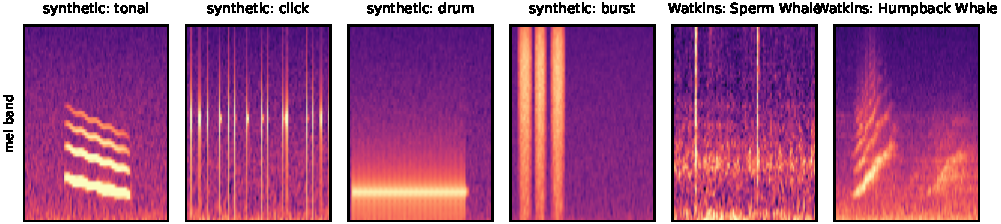
\includegraphics[width=\textwidth]{figures/clips.pdf}
\caption{Log-mel clips (64 bands $\times$ 96 frames, 2\,s). Four synthetic
call families at 5\,km range under Wenz noise, and two real Watkins clips.}
\label{fig:clips}
\end{figure*}

\subsection{A synthetic deep-sea soundscape}
A \emph{species} is a call family with a species-specific parameter
distribution, narrow enough that two species of the same family differ in a
stable way: \emph{tonal} (FM sweep with harmonics and vibrato; baleen moans,
whistles), \emph{click} (train with a characteristic inter-click interval and
centre frequency), \emph{drum} (pulsed swim-bladder knocks) and \emph{burst}
(band-limited noise pulses). Each clip draws a call realisation with $\pm12$\%
parameter jitter, scales it to the species' source level (150--185\,dB re
1\,$\mu$Pa), applies the transmission loss of Section~\ref{sec:budget} at a
log-uniform range of 1--100\,km, and adds Gaussian noise shaped by the Wenz
spectrum at sea state 3. Features are 64-band log-mel spectrograms of 2\,s at
16\,kHz (Figure~\ref{fig:clips}). The local study uses \NovNKnown\ known and
\NovNUnknown\ unknown species with \NovClips\ clips each (mean receiver SNR
\NovSnrBase\,dB).

\subsection{Real calls}
The Watkins Marine Mammal Sound Database ``best of'' cuts, in the BEANS
packaging \cite{hagiwara2022beans}, provide \RealClips\ clips of
\RealSpecies\ species with at least eight clips each (two of the four parquet
shards). Clips are resampled to 16\,kHz, cropped or padded to 2\,s and
featurised identically; a small quantised cache is checked in so the pipeline
reproduces offline.

\subsection{Models and novelty scores}
A three-block CNN (16--32--64 channels, global pooling, 64-d embedding,
softmax head) is trained with cross-entropy on the known species only; a
convolutional autoencoder (32-d latent) is trained on the same clips; and a
PCA(40) + multinomial logistic pipeline is the shallow baseline. On held-out
known clips and all unknown clips we compute six novelty scores: $1-\max$
softmax \cite{hendrycks2017baseline}, energy $-\log\sum e^{z}$
\cite{liu2020energy}, cosine distance to the $k$-th nearest training embedding
($k=5$) \cite{sun2022knn}, minimum class-conditional Mahalanobis distance
\cite{lee2018simple}, autoencoder reconstruction error, and $1-\max$ probability
of the PCA baseline. Metrics are AUROC and AUPR for unknown-vs-known and the
false-positive rate at 95\% recall of unknowns, plus the known-class accuracy.

\subsection{From novel clips to candidate species}
Clips whose score exceeds the \CluFlagQ th percentile of the known test scores
are flagged; their embeddings are clustered by average-linkage agglomerative
clustering on cosine distance, with the number of clusters chosen by the
silhouette score over 2--10. We report the adjusted Rand index against the true
unknown-species labels, the estimated versus true number of new species, and
the precision and recall of the flagging step.
